\chapter{Models@Runtime for the IoT}
\label{ch:MARContiki}
As presented in chapter \ref{ch:IoT}, Internet of Things systems are typically formed by a myriad of many small interconnected devices.
This underlying hardware infrastructure raises new challenges in the way we administrate the software layer of these systems.
Indeed, the limited computing power and battery life of each node combined with the very distributed nature of these systems, greatly adds complexity to distributed software layer management.

In this chapter, I describe a first approach to implement a new middleware dedicated to IoT devices, in order to enable the management of software deployment and the dynamic reconfiguration of IoT systems.
Our middleware is inspired from the Component Based Systems and the model@runtime paradigm which have been already described in the previous chapter.
Moreover, the implementation of this middleware follows the directions of the existing Kevoree meta-model\todo{\cite{}}, which has been adapted to fit IoT devices constraints. 
The evaluation of these constraints were conducted on several hardware platforms typical of the IoT, in order to establish a reference for the minimum requirements to run such a middleware.
Once an initial research on these IoT platforms was conducted, the proposition of a new one was necessary, since the minimal requirements were not met by the commercially available platforms at that time.
Such platform was an essential part to evaluate our first implementation, and was used to establish the minimum requirements of an execution environment.
Finally, we have conducted an initial evaluation on an Internet of Things testbed\cite{Fleury15iotlab} recently available for experimentation.
Our results demonstrates the feasibility of providing a model@runtime middleware for these systems, which can be executed in platforms meeting the requirements already established.
This chapter is concluded by the obtained results in the FIT IoT-Lab testbed, which show the limits of our first approach.

\section{Overview}
%context
Nowadays, we are surrounded by a plethora of interconnected devices (mobile phones, household appliances, wearable sensors, and so on) that continuously collect data on our living environment.
This distributed computing infrastructure is becoming pervasive and users tend to naturally interact with it. This new computing environment offers a lot of opportunities for developing new applications in many different domains.
Technology can now operate behind the scene by dynamically responding to people wishes.
Based on this principle, IoT dedicated devices have emerged, forming the IoT infrastructure already described in section \ref{sec:IoTInfra}.
All this new IoT devices form a constellation of many small interconnected objects integrated into houses, building, cities, factory chain, etc.
%Based on this principle, Cyber Physical Systems (CPS) have emerged.CPS are pervasive and long living systems formed by a constellation of many small interconnected devices integrated into houses, building, cities, factory chain, etc. 

%motivation
In our building automation scenario presented in section \ref{sec:BAScenario}, the described IoT subsystem typically rely on sensor nodes that detect and record data such as presence, temperature, ambient lighting and energy consumption. 
Thus, the IoT uses sensors to continuously analyse the situation in order to adapt our living environment to match user needs and preferences.
User wishes may involve different objectives such as comfort, air quality, and energy savings. 
To go beyond energy management and comfort, building automation systems have to deal with new types of services, depending on the use of the building: fire safety and security management for hotel, indoor air quality control in schools and office buildings, etc. 
The opportunities of services offered by the IoT and the user preferences are countless and will change over the lifetime of these systems.
The set of small interconnected devices integrated into building can be seen as a computing infrastructure that can host these new services. 
Consequently the software deployed on these nodes needs to be dynamically reconfigured and re-deployed to meet the evolution of services and user preferences. 

% old sentences
%Consequently comfort and quality are factors of productivity and do not prevent energy savings being achieved.
%To go beyond energy management, building automation systems have to deal with new types of services, depending on the use of the building: fire safety and security management for hotel, indoor air quality control in schools and office buildings etc. 


%problem
For this reason, the capacity of dynamically deploying and reconfiguring the software layer of the IoT is a crucial feature.
We address the problem of enabling the deployment of a distributed software layer and its dynamic reconfiguration over a network of nodes featuring very limited resources: memory, processing power, bandwidth communication and energy autonomy. 

% limitation of SOTA
To solve this problem, various techniques have been proposed, such as system image replacement \cite{hui2004dynamic} and virtual machines \cite{koshy2005vmstar}. 
These approaches have two main drawbacks. 
First they are not efficient in terms of energy. 
Second, while they are suited to deploy static applications, these are not convenient solutions for IoT, since IoT devices operates in dynamic environments in which tasks performed by each node must be easily and frequently adapted.

%our approach
In this chapter we present our initial results towards the design of a middleware featuring deployment and reconfiguration facilities over an IoT system. 
Our middleware aims at implementing the paradigm of model@runtime taking into account the stringent requirements of IoT devices.

%plan
%This paper is structured as follows. Section 2 presents the Kevoree component model. Section 3 details the challenges of mapping the model@runtime paradigm to microcontrollers, and explains how we implemented Kevoree on these very limited nodes. Our proposal is evaluated in section 4. Section 5 presents related work and Section 6 gives our conclusion and highlights some perspectives to be addressed in future work.

\section{A M@R approach for constrained IoT devices}
The model@runtime paradigm has been mainly investigated in the context of distributed systems. 
These research efforts have been focused on the provision of a comprehensive set of tools to easily deploy, dynamically reconfigure, and disseminate software on a set of distributed computing units.
The current model@runtime tools have been implemented regardless of the specific characteristics and constraints of IoT devices.
In particular, the network topology and the resource constraints of the nodes forming the distributed system have not been taken into consideration.
As a result, state of the art model@runtime tools are not suitable to be used in the context of IoT Systems.
First, most approaches are relying on the Java language, which does not meet the resource constraints of the computing nodes. 
Secondly, the size of the model and its distribution among the system are not taking into consideration the limited memory capacity of each node, and their energy constraints.

In \cite{fouquet2012dynamic}, an effort has been made to port the model@runtime paradigm on the constraints of a Cyber Physical System (CPS), in which the underlying device is comparable to an IoT device.
Despite the particular attention given to the specific constraints of a Cyber Physical System, this work heavily relies on over the air firmware flashing to support the deployment and reconfiguration of software. 
We consider that relying on firmware flashing to support software deployment constitutes a flaw in the approach because of its energy cost (the complete firmware has to be sent, and if any error occurs, the whole process is restarted).
A second limitation of this approach lies in the fact that each resource constrained node relies on a more powerful node to perform most of his task related to the dynamic reconfiguration (firmware synthesis, reconfiguration decision and so on).
This second limitation is not suitable in the context of a system mainly composed of resource constrained nodes since all the resource constrained nodes have to be managed by bigger nodes.
Pushing this idea further, the management of a CPS composed of a wide number of resource constrained devices and a bigger node, the latter will have to manage all the smaller devices in a centralized management scheme.

Therefore, a new approach implementing a more complete M@R engine has been proposed.
The next section will describe an implementation based on the Kevoree meta-model, together with some tools which allow model manipulation.

\subsection{Our M@R implementation}
\label{subsec:MARImpl}
Since our work aims to provide a M@R engine for IoT devices, a first implementation should be developed having in mind the programming constraints.
Taking into account this limitations means that, first of all, we must fit the programming constraints.
In contrast with most of the current implementations of the M@R paradigm, which are intended for high resources machines thus they make use of high-level programming languages, our first implementation should follow a procedural language such as C.
We can justify this by the fact that most of the open source compilers for IoT devices support only this programming language, in addition to C++.
However, C++ applications are difficult to integrate in OSs like Contiki, which is one of the most convenient OS able to run our middleware.
Thus, a first approach has been developed in plain C\footnote{\url{https://github.com/kYc0o/kevoree-c}}.
This raised big challenges since the object-oriented meta-model representation is very difficult to transform into C structures, knowing that there is no modeling framework supporting such a language.

\begin{table}[]
	\centering
	\caption{Size of a plain C minimalistic Kevoree meta-model implmentation}
	\label{tab:kevoreeC}
	\begin{tabular}{cccccc}
		\texttt{text}   & \texttt{data} & \texttt{bss} & \texttt{dec}    & \texttt{hex}   & \texttt{filename} \\
		\texttt{181997} & \texttt{1448} & \texttt{168} & \texttt{183613} & \texttt{2cd3d} & \texttt{main}        
	\end{tabular}
\end{table}

\begin{figure}[]
	\centering
	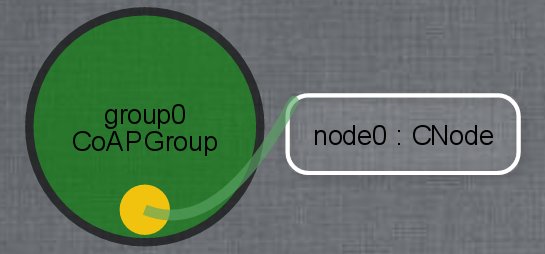
\includegraphics[width=0.55\columnwidth]{chapters/modelsAtRuntimeContiki.images/1stModel.png}
	\caption{Graphical representation of a minimal M@R}
	\label{fig:1stModelC}
\end{figure}

Thus, our efforts were  to a first manual implementation of the Kevoree meta-model.
The size of the test application which contains a group and a node without components is shown in table \ref{tab:kevoreeC}
A graphical representation of the model can be obtained through the Kevoree Web Editor\footnote{\url{http://editor.kevoree.org/v4/}}, in which a serialized JSON file containing the model can be loaded for edition.
This representation is shown in figure \ref{fig:1stModelC}.

Our firsts results show that approximately 180KB of ROM space (text) are needed for the implementation, while 14KB of RAM (data + bss) were enough for such application.
This test was compiled using the GCC (GNU C Compiler) version 4.9, for a i386 32-bit platform.
Therefore, we need to find an IoT device which fit this minimal requirements.

It is then necessary to characterize the minimum system requirements for an IoT device to implement a full model@runtime middleware, as in hardware capabilities as in execution environment.
This will avoid the use of third party nodes to perform the high level tasks described above.
However, even if a proposed device meet the characteristics to perform such tasks, the trade-offs between energy consumption and the middleware execution should be taken into account.
A general description of needed features to execute the proposed middleware is given in the next subsection.

%\subsection{Needed features of the underlying system}
\subsection{Kevoree-IoT operating system requirements}
Our middleware approach, which is called Kevoree-IoT (in reference to the kevoree-like M@R implementation of our middleware), will need several features proposed by the underlying system.
As we discussed previously, the most common approach used to run applications in IoT devices is bare-metal development followed by firmware flashing into the ROM memory.
Even if this method allows a fine control of the underlying hardware, the development time can be very long and difficult to debug, since abstractions are mostly done only at the hardware level, and does not come to the system level.
As the complexity grows, applications for IoT should be developed without special attention to hardware and system concerns.
Thus, an IoT operating system should be used, in order to leverage its system-level abstractions.
As presented in the state of the art, several IoT operating systems exist, but according to the needed features we should make a choice.
This features are the following:
\begin{enumerate}
	\item \textbf{Network stack implementing basic IP functions (TCP, UDP, HTTP, CoAP).} In order to share a m@r and download software artifacts, IP communication is mandatory, since the goal is to use the Internet to reach devices from different domains.
	\item \textbf{Persistent data handling, preferably a file system.} The method used to represent a m@r is using serialized objects, usually in the JSON format. Thus, a way to store this JSON file should be provided.
	\item \textbf{Dynamic linker and loader, following the third approach presented in section \ref{sec:IoTDeployment}.} A dynamic linker and loader is essential to our approach, since changes in the model containing new software components will trigger the download and instantiation of an artifact, which should be linked and loaded at runtime by the underlying system.
	\item \textbf{Abstractions for attached devices (LEDs, sensors, actuators, etc.).} Although not mandatory, an OS usually carry basic hardware abstractions, providing an easy way to develop applications which need a physical connection with the external world.
	\item \textbf{Basic OS functionalities such as timers, task scheduler and Inter Process Communication (IPC).} Basic functionalities that are implemented very often by almost any OS.
\end{enumerate}
Given the features presented above, the system which fits all the requirements is the Contiki OS.
Despite the programming model already described as a drawback, Contiki offers all the needed functionalities, as well as a wide community which collaborate very actively in the development and debug of it.
Therefore, we use the ContikiOS\cite{dunkels2004contiki} in order to provide an efficient way to distribute components, since it allows dynamic loading of binary modules.
Contiki includes an implementation of the IPv6 compressed stack, 6loWPAN\cite{rfc4944}, which let us assign directly an IPv6 address. 
This enables a ready to use IoT environment.
We use erbium's\cite{rfc7252} CoAP implementation in order to have a REST engine which enables services discovery through the network.
It is also used as a main communication channel between nodes. The dynamic code loading mechanisms are based on a dynamic linker and loader that use the standard ELF object file format\cite{dunkels06runtime}.

The first implementation\footnote{\url{https://github.com/kYc0o/kevoree-contiki}} is done using the version 4 of the Kevoree meta-model.
This meta-model has been mapped into C code as a Contiki application.
We are able to add nodes, components, groups and channels, and bind them through the Kevoree editor loading a generated JSON file.

However, even if the OS fulfill all the requirements, the computational resources needed by our middleware should be taken into account, in order to find a platform on which we can evaluate our approach.


\subsection{Handling hardware constraints}
Designing the presented middleware in the context of the IoT raises scientific challenges.
All the following challenges are related to the limited resources of these nodes and the particular topology of the network that interconnect them.

Currently the concept of model@runtime has been applied on top of object oriented languages which offers the required features at the language level to implement the model@runtime layer. 
The first challenge lies in the fact that Contiki does not support these object oriented languages and thus the design must fit a procedural language such as C.

The second challenge lies in the very limited resources of the IoT nodes, thus forcing the middleware to meet the memory and CPU constraints. 
This imposes constraints on the way the model is represented, stored and processed on each node.
%This challenge is particularly important and hard to meet, since many software components are needed to enable the communication in these environments (radio/MAC/IP stack and so on).
Moreover, the energy constraint of each IoT node, together with the mesh topology of the network makes communication in this environments fairly reliable.
This implies the necessity to optimize the way the model and the software are disseminated in the network.

At first glance, our implementation was tested on three different platforms: the \textit{\textbf{zolertia Z1\footnote{\url{http://zolertia.sourceforge.net/wiki/images/e/e8/Z1_RevC_Datasheet.pdf}}, redbee econotag\footnote{\url{http://redwire.myshopify.com/products/econotag-ii}} and wismote\footnote{\url{http://wismote.org/doku.php}}}}, which were widely used for research purposes in the IoT domain.
Unfortunately, none of these platforms was able to meet the space requirements in ROM and RAM to run a minimal model at runtime as shown in figure \ref{fig:1stModelC}.
However, the existence of more powerful microcontrollers, an essential part of an IoT device, shows that typical IoT applications have not exceeded the resources of existing experimentation platforms.
Indeed, only some development kits such as TI's CC2538DK\footnote{\url{http://www.ti.com/tool/cc2538dk}} were available at that time, but its high cost, low availability and poor support gave low acceptance for research purposes.
Thus, the design and construction of a new experimentation platform seemed to be the fastest way to obtain the first results of the implementation, using the latest microcontrollers and peripherals available on the market.
It is worth to consider that this platform was conceived for research and experimentation purposes, and not as an end-user device.

An exhaustive search was conducted to find the latest technologies to build an experimentation IoT device, which fits the requirements already estimated in section \ref{subsec:MARImpl}.
The first step was to find the basic components of such a device.
Taking into account the requirements, an IoT device should embed:
\begin{enumerate}
	\item \textbf{Microcontroller.} A very low-power microcontroller unit is needed to perform the computational processing tasks as well as to store the program code. 
	A huge amount of ROM and RAM is needed at the scale of these devices, thus it is necessary to find a microcontroller with a good trade-off between energy consumption and memory size.
	\item \textbf{Communication interface.} Communication is the main task that will perform our device, since it is mandatory for IoT environments.
	A radio interface implementing the widely used IEEE 802.1.5.4 standard\cite{ieee802.15.4} is then necessary to communicate in an interoperable way with other devices.
	An ultra-low energy consumption is also important, since communication is the most energy consuming task.
	\item \textbf{External flash memory.} Storage for data is a very useful feature for an IoT device. It can serve as persistent data storage for logging and data collection from sensors, as well as updates and eventually new firmwares.
	\item \textbf{Sensors and actuators.} In order to collect experimentation data, some sensors should be embedded on the device, the most common being temperature, humidity and position.
	Indicator LEDs are also commonly present in these devices, to provide visual signs such as function status (ON/OFF) or current communication.
	\item \textbf{Ports for external devices.} An easy way to connect third party devices allows a dynamic behavior, since we can connect other sensors, actuators and devices which cannot be present internally on the device.
	Such devices should be connected using standard interfaces, such as I2C and SPI.
	General Purpose Inputs/Outputs (GPIO) are also widely used, either as digital or analog interfaces.
	\item \textbf{Battery capabilities.} An IoT device is very often used in environments where a constant power source is not present.
	Thus, work on batteries is a very useful feature to test energy consumption while adding flexibility of placement.
\end{enumerate}

Given these features, it was then necessary to integrate several components in order to build the required IoT device.
We put special attention to the most critical components, which are the microcontroller, the external flash memory and the battery controller.
Regarding the radio transceiver and the other peripherals, there are no huge differences between the most commonly used, for instance, the ones used in the previously tested devices.
The specific conception of the platform will be described in the next subsection.

\subsection{Towards a new IoT device}

Several low-power microcontroller architectures were available at the time of our first M@R implementation, such as TI MSP430, Atmel AVR, Microchip PIC and ARM Cortex-M, just to mention the most common ones.
Since our middleware minimum memory requirements were tested on 16-bit MSP430 microcontrollers (Zolertia's Z1 and Arago's WiseMote) finding a huge scarcity of memory, 32-bit architectures were the target of our scope.
Indeed, ARM Cortex-M microcontrollers offer only 32-bit RISC architectures, which are widely used both in research and industry.
Thus, the first step was to select an ARM Cortex-M microcontroller fitting our memory and energy consumption requirements.
The STM32 family of microcontrollers offers a wide range of devices with different processor speeds and memory sizes.
\begin{figure}[]
	\centering
	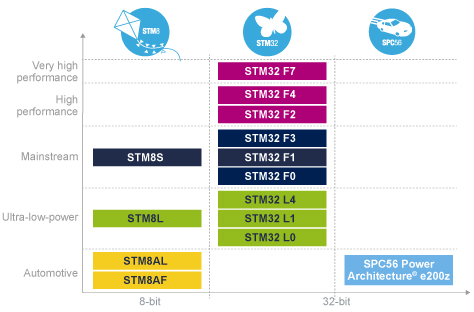
\includegraphics[width=0.70\columnwidth]{chapters/modelsAtRuntimeContiki.images/STM32.jpg}
	\caption{STM32 Microcontroller family}
	\label{fig:STM32}
\end{figure}
Figure \ref{fig:STM32} shows the STM32 family applications and available solutions for each one.

At the time of this search, ultra-low-power solutions (STM32L) were not available, thus our possibilities were in the STM32F range, excluding the F7 which was also recently released.

\begin{table}[]
	\centering
	\caption{Comparison between STM32F microcontrollers}
	\label{tab:STM32F}
	\begin{tabular}{c|cccc}
		Microcontroller & Speed (MHz) & RAM (KB) & ROM (KB) & \begin{tabular}[c]{@{}c@{}}Consumption \\ at max. speed (mA)\end{tabular} \\ \hline
		STM32F0         & 48          & 32       & 256      & 22                                                                        \\
		STM32F1         & 72          & 96       & 1024     & 68                                                                        \\
		STM32F3         & 72          & 80       & 512      & 61.5                                                                      \\
		STM32F2         & 120         & 128      & 1024     & 49                                                                        \\
		STM32F4         & 180         & 256      & 2048     & 98                                                                       
	\end{tabular}
\end{table}

Since our goal is to build a device on which our experimentations could be executed in a more flexible way (without caring about memory requirements), it is preferable to use a microcontroller featuring the highest memory, both in ROM and RAM, over energy consumption.
Moreover, these kind of devices are able to change the processor speed as needed, thus reducing the energy consumption.
Therefore, the STM32F4 microcontroller was used as the core of our IoT device.
Table \ref{tab:STM32F} shows a comparison between the available microcontrollers, featuring the maximum processor speed, RAM and ROM, followed by the current consumption in such configuration.

As for the power scheme, given the capabilities of the selected microcontroller, a power source between 1.8V and 3.6V is required.
Indeed, a first approach to power the device is the use of an USB port, which delivers around 5V.
Thus, a 5V to 3.3V (the recommended tension) is required.
In contrast, when the device is needed to run on batteries, the supplied voltage will change.
The most common batteries available on the market provide between 1.5V (AA, AAA) and 3V (CR3032), which is in the acceptable range.
A couple of 2 AA batteries connected in series is the most standard array to power IoT devices, delivering 3V, enough for our device.
However, a wide set of peripherals such as sensors and actuators work very often at 5V.
Therefore, it was necessary to add a DC to DC converter, coupled with an automatic switch to detect when the device is powered either by USB or batteries.
This allows to use any power scheme without decreasing performance or peripherals compatibility.

\begin{table}[]
	\scriptsize
	\centering
	\caption{IoT Platforms comparison}
	\label{tab:IoTPlatfComp}
	\begin{tabular}{cccccccc}
		\textbf{}                                                                               & \textbf{\begin{tabular}[c]{@{}c@{}}Speed \\ (MHz)\end{tabular}} & \textbf{\begin{tabular}[c]{@{}c@{}}RAM \\ (KB)\end{tabular}} & \textbf{\begin{tabular}[c]{@{}c@{}}ROM \\ (KB)\end{tabular}}                               & \textbf{\begin{tabular}[c]{@{}c@{}}External \\ flash (MB)\end{tabular}} & \textbf{\begin{tabular}[c]{@{}c@{}}Radio \\ transceiver\end{tabular}} & \textbf{Peripherals}                                                                                    & \textbf{\begin{tabular}[c]{@{}c@{}}Embedded\\ Sensors\end{tabular}}                                \\ \cline{2-8} 
		\multicolumn{1}{c|}{\textbf{\begin{tabular}[c]{@{}c@{}}Zolertia \\ Z1\end{tabular}}}    & \multicolumn{1}{c|}{16}                                         & \multicolumn{1}{c|}{8}                                       & \multicolumn{1}{c|}{96}                                                                    & \multicolumn{1}{c|}{2}                                                  & \multicolumn{1}{c|}{CC2420}                                           & \multicolumn{1}{c|}{\begin{tabular}[c]{@{}c@{}}UART, I2C\\ Phidgets \\ (USB only),\\ GPIO\end{tabular}} & \multicolumn{1}{c|}{\begin{tabular}[c]{@{}c@{}}3 axis acc.\\ and\\ temperature\end{tabular}}       \\ \cline{2-8} 
		\multicolumn{1}{c|}{\textbf{\begin{tabular}[c]{@{}c@{}}Arago's\\ WisMote\end{tabular}}} & \multicolumn{1}{c|}{25}                                         & \multicolumn{1}{c|}{16}                                      & \multicolumn{1}{c|}{256}                                                                   & \multicolumn{1}{c|}{8}                                                  & \multicolumn{1}{c|}{CC2520}                                           & \multicolumn{1}{c|}{\begin{tabular}[c]{@{}c@{}}UART, I2C,\\ Phidgets, \\ GPIO\end{tabular}}             & \multicolumn{1}{c|}{\begin{tabular}[c]{@{}c@{}}3 axis acc.\\ light and\\ temperature\end{tabular}} \\ \cline{2-8} 
		\multicolumn{1}{c|}{\textbf{\begin{tabular}[c]{@{}c@{}}Redbee\\ econotag\end{tabular}}} & \multicolumn{1}{c|}{26}                                         & \multicolumn{1}{c|}{96}                                      & \multicolumn{1}{c|}{\begin{tabular}[c]{@{}c@{}}N/A\\ (device run\\ from RAM)\end{tabular}} & \multicolumn{1}{c|}{128 (KB)}                                           & \multicolumn{1}{c|}{Integrated (SoC)}                                 & \multicolumn{1}{c|}{GPIO}                                                                               & \multicolumn{1}{c|}{N/A}                                                                           \\ \cline{2-8} 
		\multicolumn{1}{c|}{\textbf{\begin{tabular}[c]{@{}c@{}}DiverSE\\ Board\end{tabular}}}   & \multicolumn{1}{c|}{180}                                        & \multicolumn{1}{c|}{256}                                     & \multicolumn{1}{c|}{2048}                                                                  & \multicolumn{1}{c|}{16}                                                 & \multicolumn{1}{c|}{CC2520}                                           & \multicolumn{1}{c|}{\begin{tabular}[c]{@{}c@{}}UART (x2), \\ I2C\\ Phidgets, \\ GPIO\end{tabular}}      & \multicolumn{1}{c|}{N/A}                                                                           \\ \cline{2-8} 
	\end{tabular}
\end{table}

Thus far, the main required features for our device are met.
A comparison between the previously tested platforms and ours is given in table \ref{tab:IoTPlatfComp}, showing the most common useful features.
Details about the other components such as the radio transceiver and the external flash memory can be found in annex X.



\subsection{Kevoree-IoT Contiki implementation}

%\subsubsection{First experiences with a new hardware platform}


\section{A large-scale platform for validation}

\subsection{FIT IoT-Lab}

\subsection{Extending the testbed}

\subsubsection{File system driver implementation}

\subsubsection{Runtime address relocation for ARM Cortex-M3 platforms}

\section{M@R experiment results in the IoT-Lab testbed}